\chapter{Технологическая часть}

В данном разделе описаны инструменты, использованные для реализации, а также представлены листинги трёх алгоритмов.

\section{Средства реализации}
Для реализации был выбран язык C++ в качестве среды разработки использовалась Visual Studio Code с компилятором g++. Для модульного тестирования применялась библиотека Check, а для визуализации результатов~--- утилита gnuplot~\cite{mscpp}


\section{Реализация алгоритмов}

Реализация алгоритма полного перебора представлена в листинге~\ref{lst:brut}.

Реализация алгоритма выбора следующего города приведена в листинге~\ref{lst:city}.

Реализация муравьиного алгоритма представлена в листинге~\ref{lst:ant}.

\section{Демонстрация работы программы}

Демонстрация работы программы представлена на рисунке~\ref{fig:picture}

\begin{figure}[h!]
	\centering
	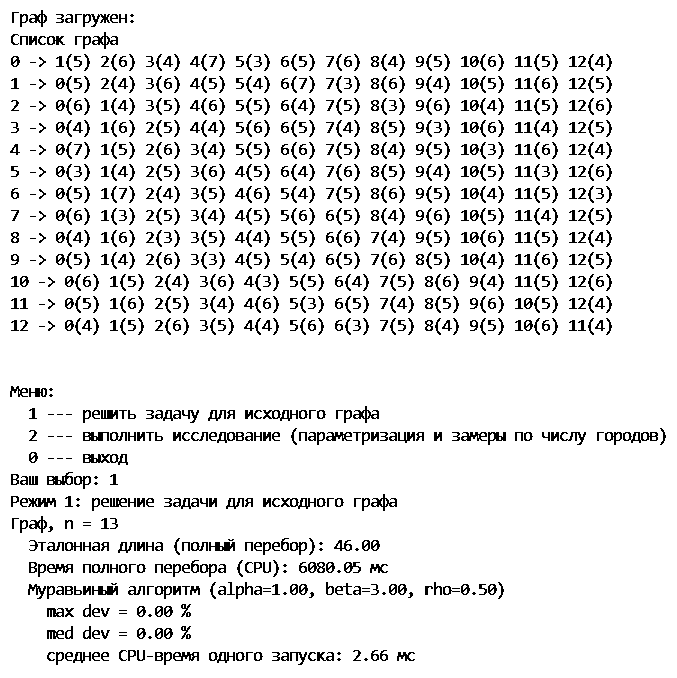
\includegraphics[width=0.7\textwidth]{images/picture.png}
	\caption{Демонстрация работы программы}
	\label{fig:picture}
\end{figure}


\clearpage
\section{Функциональные тесты}



Для проверки корректности реализации алгоритмов были проведены функциональные тесты, представленные в таблице~\ref{tab:functional-tests}.

\begin{table}[H]
	\centering
	\caption{Функциональные тесты алгоритмов поиска гамильтонова цикла}
	\label{tab:functional-tests}
	\renewcommand{\arraystretch}{1.25}
	\begin{tabular}{|c|p{4.2cm}|p{3cm}|p{3cm}|p{3cm}|}
		\hline
		\textbf{№} &
		\textbf{Входной граф} &
		\textbf{Ожидаемый результат} &
		\textbf{Полный перебор} &
		\textbf{Муравьиный алгоритм} \\ \hline
		
		1 &
		$n=4$ \newline
		1->2(10), 3(15), 4(20); 2->1(10), 3(35), 4(25); 3->1(15), 2(35), 4(30); 4->1(20), 2(25), 3(30)
		&
		Путь: [1, 2, 4, 3] \newline Стоимость: 65
		&
		Путь: [1, 2, 4, 3] \newline Стоимость: 65
		&
		Путь: [1, 2, 4, 3] \newline Стоимость: 65
		\\ \hline
		
		2 &
		$n=3$ \newline
		1->2(1), 3(2); 2->1(1), 3(3); 3->1(2), 2(3)
		&
		Путь: [1, 2, 3] \newline Стоимость: 4
		&
		Путь: [1, 2, 3] \newline Стоимость: 4
		&
		Путь: [1, 2, 3] \newline Стоимость: 4
		\\ \hline
		
		3 &
		$n=4$ \newline
		1->2(5), 3(10), 4(8); 2->1(5), 3(6), 4(9); 3->1(10), 2(6), 4(4); 4->1(8), 2(9), 3(4)
		&
		Путь: [1, 2, 3, 4] \newline Стоимость: 15
		&
		Путь: [1, 2, 3, 4] \newline Стоимость: 15
		&
		Путь: [1, 2, 3, 4] \newline Стоимость: 15
		\\ \hline
		
	\end{tabular}
\end{table}






\section*{Вывод}
В данном разделе были представлены средства реализации, реализации алгоритмов и функциональные тесты.


